\documentclass{beamer}
\usepackage{listings}
\lstset{
language=C,
frame=single, 
breaklines=true,
columns=fullflexible
}
\usepackage{subcaption}
\usepackage{url}
\usepackage{tikz}
\usepackage{graphicx}
\usepackage{multicol}
\usepackage{tkz-euclide} % loads  TikZ and tkz-base
%\usetkzobj{all}
\usetikzlibrary{calc,math}
\usetikzlibrary{shapes,arrows.meta,automata, positioning}
\usepackage{float}
\usepackage{amsthm}
\newcommand\norm[1]{\left\lVert#1\right\rVert}
\renewcommand{\vec}[1]{\mathbf{#1}}
\newcommand{\R}{\mathbb{R}}
\newcommand{\C}{\mathbb{C}}
\newcommand{\comb}[2]{{}^{#1}\mathrm{C}_{#2}}
\providecommand{\brak}[1]{\ensuremath{\left(#1\right)}}
\providecommand{\abs}[1]{\vert#1\vert}
\providecommand{\fourier}{\overset{\mathcal{F}}{ \rightleftharpoons}}
\providecommand{\sbrak}[1]{\ensuremath{{}\left[#1\right]}}
\usepackage[export]{adjustbox}
\usepackage[utf8]{inputenc}
\usepackage{amsmath}
\usepackage[version=4]{mhchem}
\usetheme{Boadilla}
\title{Dynamic Bandwidth Allocation in GMPLS Optical Networks using Minimum Execution Time Technique}
\author{Srivatsan T}
\institute{IITH}
\date{\today}
\begin{document}
\begin{frame}
  \titlepage
\end{frame}
\begin{frame}{GMPLS - Generalised MPLS}
  \begin{block}{MPLS-Multi Protocol Label Switching}
    \begin{enumerate}
      \item Traditional IP methods used routing tables and destination IP's to route incoming packets.
      \item MPLS uses LSP (Label Switched paths) and reduces reliance on routing tables.
      \item MPLS is protocol independent
    \end{enumerate}
  \end{block}
\end{frame}
\begin{frame}{MPLS in action}
  \begin{figure}[!]
    \centering
    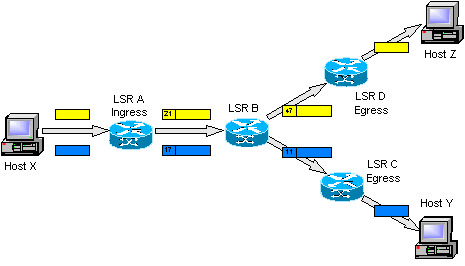
\includegraphics[width = 0.8\columnwidth]{MPLS-diagram.jpg}
    \caption{Label switching in MPLS connections}
  \end{figure}
\end{frame}
\begin{frame}{GMPLS}
  GMPLS uses implicit labels generated from the incoming packets itself
  \begin{block}{}
    \begin{enumerate}
      \item Timeslot to identify the LSP, on a Time Division Multiplexed (TDM) link
      \item Wavelength to identify the LSP, on a Wavelength Division Multiplexed (WDM) link
      \item Fiber or port on which a packet is received.
    \end{enumerate}
  \end{block}
  LSP traffic is switched based on a continuous, constant property of the data stream –
  making GMPLS a highly suitable protocol to run in high bandwidth networks.
\end{frame}
\begin{frame}{Blocking Probability}
  \begin{block}{Blocking-Definition}
    Blocking in telecommunication systems is when a circuit group is fully occupied and unable to accept further calls.
  \end{block}
  This can be handled in 2 ways
  \begin{block}{}
    \begin{enumerate}
      \item Unconnected users can be queued and connected again when servers are free
      \item Unconnected user details can be cleared which leads to the call never being connected
    \end{enumerate}
  \end{block}
\end{frame}
\begin{frame}{Blocking Probability}
  \begin{block}{Blocking probability-Definition}
    The probability that the call being made is not successfully connected immedietly. Alternatively it is
    the probability that the call being made by the user is either queued or cleared.
  \end{block}
  To improve quality of service (QoS) it is essential to minimize Blocking probability as much as we can.
\end{frame}
\begin{frame}{Calculation of Blocking Probability}
  Let us first define some variables
  \begin{block}{Variables}
    \begin{enumerate}
      \item N - Total number of servers available
      \item $\lambda$ - mean call arraival rate
      \item Let the call timings be exponentially distributed with $\frac{1}{\mu}$ as its mean
      \item $\mu$ - mean calls completion rate
    \end{enumerate}
  \end{block}
\end{frame}
\begin{frame}{Poisson's Distribution}
  Number of calls arrived and completed is modelled as a poisson random variable
  \begin{block}{Call Arrival}
    P(m calls generated in time T) = $\frac{{(\lambda T)^m}}{m!}$ $e^{-\lambda T}$
  \end{block}
  \begin{block}{Call completion}
    P(m calls completed in time T) = $\frac{{(\mu T)^m}}{m!}$ $e^{-\mu T}$
  \end{block}
\end{frame}
\begin{frame}{Concept of Traffic}
  \begin{block}{Definition}
    Offered Traffic is a measure of the number of concurrent calls that could be carried by the network if
    there were no restrictions on the number of servers.It is expressed in Erlangs (dimension less)
  \end{block}
  It is calculated by finding the busiest hour of the day and multiplying the average call time in that hour (in hours)
  and the number of calls that arrived in that hour.
  \begin{block}{Formula}
    Offered Traffic A = $\lambda \times \frac{1}{\mu}$ Erlangs
  \end{block}
\end{frame}
\begin{frame}{Erlang B Queuing model}
  \begin{block}{}
    In the Erlang B queueing model, customers arrive at a queueing system having n servers but having 0 waiting positions.
    We assume Poisson arrivals and exponentially distributed service times.
    Since there are no waiting positions, it is understood that if a customer finds upon arrival that
    no servers are available, then the customer goes away and is lost.
  \end{block}
\end{frame}
\begin{frame}{Birth Death Process}
  \begin{block}{Definition}
    It is a kind of process in which there are only 2 possibilities for a system. It can either have a Birth
    which increments the state variable by 1 or it can have a Death which decrements the state variable by 1.
  \end{block}
  \begin{block}{}
    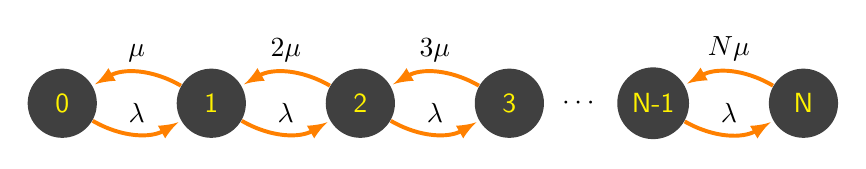
\begin{tikzpicture}[font=\sffamily]
      % Add the states
      \node[state,
        text=yellow,
        draw=none,
        fill=gray!50!black] (s) {0};
      \node[state,
        right=1cm of s,
        text=yellow,
        draw=none,
        fill=gray!50!black] (r) {1};
      \node[state,
        right=1cm of r,
        text=yellow,
        draw=none,
        fill=gray!50!black] (t) {2};
      \node[state,
        right=1cm of t,
        text=yellow,
        draw=none,
        fill=gray!50!black] (v) {3};
      \node[draw=none,  right=0.1cm of v]  (dots)  {$\cdots$};
      \node[state,
        right=0.1cm of dots,
        text=yellow,
        draw=none,
        fill=gray!50!black] (k) {N-1};
      \node[state,
        right=1cm of k,
        text=yellow,
        draw=none,
        fill=gray!50!black] (m) {N};
      % Connect the states with arrows
      \draw[every loop,
        auto=right,
        line width=0.5mm,
        >=latex,
        draw=orange,
        fill=orange]
      (s) edge[bend right, auto=left]  node {$\lambda$} (r)
      (r) edge[bend right, auto=right] node {$\mu$} (s)
      (r) edge[bend right, auto=left]  node {$\lambda$} (t)
      (t) edge[bend right, auto=right] node {$2\mu$} (r)
      (t) edge[bend right, auto=left]  node {$\lambda$} (v)
      (v) edge[bend right, auto=right] node {$3\mu$} (t)
      (k) edge[bend right, auto=left]  node {$\lambda$} (m)
      (m) edge[bend right, auto=right] node {$N\mu$} (k);
    \end{tikzpicture}
  \end{block}
  \bigskip
  Let $P_k$ denotes the probability that there are k callers in the system.
\end{frame}
\begin{frame}{Birth-Death Contd.}
  \begin{block}{}
    \begin{center}
      $P_1 \mu = P_0 \lambda$\\
      This can be generalised as follows\\
      $P_k \hspace{0.2cm} k\mu = P_{k-1} \hspace{0.2cm} \lambda \hspace{0.5cm} 1 \leq k \leq N$
    \end{center}
  \end{block}
  Which gives,
  \begin{align}
    P_k = \frac{\lambda}{k\mu} P_{k-1} = \frac{\lambda^2}{k(k-1)\mu} P_{k-2} = \cdots = \frac{1}{k!} \brak{\frac{\lambda}{\mu}}^{k} P_0
  \end{align}
  We can calculate $P_0$ using the normalisation condition $\sum_{k = 0}^{N} P_k = 1$\\
  Replacing $\frac{\lambda}{\mu}$ with offered traffic A, We get the Blocking Probability as follows
  \begin{align}
    P_B = \frac{\frac{A^{N}}{N!}}{\sum_{k = 0}^{N} \brak{\frac{A^k}{k!}}}
  \end{align}
\end{frame}
\begin{frame}{Erlang C Queuing Model}
  \begin{block}{Definition}
    In the Erlang C queueing model, customers arrive at a queueing system having n servers and q waiting positions.  We also assume Poisson arrivals and exponentially distributed service times.
    If all servers are busy when a user tries to make a call, he is places in the queue and the call eventually gets connected.
  \end{block}
\end{frame}
\begin{frame}{Birth Death Model}
  \begin{block}{}
    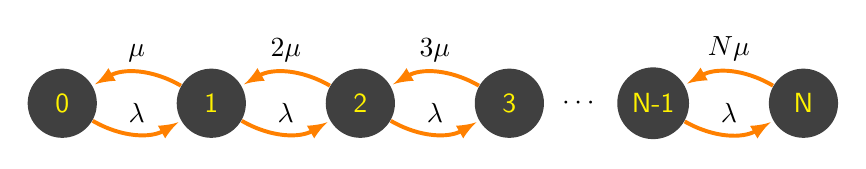
\begin{tikzpicture}[font=\sffamily]
      % Add the states
      \node[state,
        text=yellow,
        draw=none,
        fill=gray!50!black] (s) {0};
      \node[state,
        right=1cm of s,
        text=yellow,
        draw=none,
        fill=gray!50!black] (r) {1};
      \node[state,
        right=1cm of r,
        text=yellow,
        draw=none,
        fill=gray!50!black] (t) {2};
      \node[state,
        right=1cm of t,
        text=yellow,
        draw=none,
        fill=gray!50!black] (v) {3};
      \node[draw=none,  right=0.1cm of v]  (dots)  {$\cdots$};
      \node[state,
        right=0.1cm of dots,
        text=yellow,
        draw=none,
        fill=gray!50!black] (k) {N-1};
      \node[state,
        right=1cm of k,
        text=yellow,
        draw=none,
        fill=gray!50!black] (m) {N};
      % Connect the states with arrows
      \draw[every loop,
        auto=right,
        line width=0.5mm,
        >=latex,
        draw=orange,
        fill=orange]
      (s) edge[bend right, auto=left]  node {$\lambda$} (r)
      (r) edge[bend right, auto=right] node {$\mu$} (s)
      (r) edge[bend right, auto=left]  node {$\lambda$} (t)
      (t) edge[bend right, auto=right] node {$2\mu$} (r)
      (t) edge[bend right, auto=left]  node {$\lambda$} (v)
      (v) edge[bend right, auto=right] node {$3\mu$} (t)
      (k) edge[bend right, auto=left]  node {$\lambda$} (m)
      (m) edge[bend right, auto=right] node {$N\mu$} (k);
    \end{tikzpicture}
  \end{block}
  \begin{block}{}
    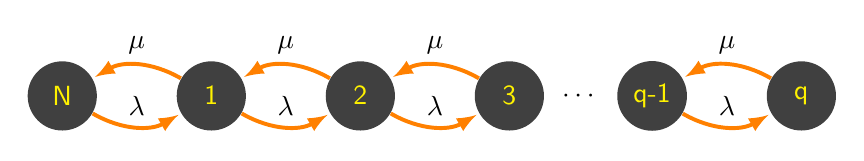
\begin{tikzpicture}[font=\sffamily]
      % Add the states
      \node[state,
        text = yellow,
        draw=none,
        fill=gray!50!black] (n) {N};
      \node[state,
        right=1cm of n,
        text=yellow,
        draw=none,
        fill=gray!50!black] (s) {1};
      \node[state,
        right=1cm of s,
        text=yellow,
        draw=none,
        fill=gray!50!black] (r) {2};
      \node[state,
        right=1cm of r,
        text=yellow,
        draw=none,
        fill=gray!50!black] (t) {3};
      \node[draw=none,  right=0.1cm of t]  (dots)  {$\cdots$};
      \node[state,
        right=0.1cm of dots,
        text=yellow,
        draw=none,
        fill=gray!50!black] (k) {q-1};
      \node[state,
        right=1cm of k,
        text=yellow,
        draw=none,
        fill=gray!50!black] (m) {q};
      % Connect the states with arrows
      \draw[every loop,
        auto=right,
        line width=0.5mm,
        >=latex,
        draw=orange,
        fill=orange]
      (n) edge[bend right, auto=left]  node {$\lambda$} (s)
      (s) edge[bend right, auto=right] node {$\mu$} (n)
      (s) edge[bend right, auto=left]  node {$\lambda$} (r)
      (r) edge[bend right, auto=right] node {$\mu$} (s)
      (r) edge[bend right, auto=left]  node {$\lambda$} (t)
      (t) edge[bend right, auto=right] node {$\mu$} (r)
      (k) edge[bend right, auto=left]  node {$\lambda$} (m)
      (m) edge[bend right, auto=right] node {$\mu$} (k);
    \end{tikzpicture}
  \end{block}
  Let $P_k$ denote the probability that there are k callers in the system.
\end{frame}
\begin{frame}{Birth Death Contd.}
  \begin{block}{}
    \begin{center}
      The regression in probaility for Erlang C queue is as follows,\\
      $P_k \hspace{0.2cm} k\mu = P_{k-1} \hspace{0.2cm} \lambda \hspace{0.5cm} 1 \leq k \leq N$\\
      $P_k \hspace{0.2cm} N\mu = P_{k-1} \hspace{0.2cm} \lambda \hspace{0.5cm} N+1 \leq  k \leq N+q$
    \end{center}
  \end{block}
  Which gives,
  \begin{align}
    P_k = P_0 \frac{A^k}{k!} \hspace{0.5cm} 0 \leq k \leq N
  \end{align}
  \begin{align}
    P_k = P_{k-1}\brak{\frac{A}{N}} =  P_{k-2}\brak{\frac{A}{N}}^2 \cdots = P_N\brak{\frac{A}{N}}^{k-N}\label{0.0.4} \\
    N+1 \leq k \leq N+q \notag
  \end{align}
\end{frame}
\begin{frame}{Blocking Probability in Erlang C Queues}
  We can replace $\eqref{0.0.4}$ with $P_N$ expression and we again use the normalisation to find $P_0$.
  \begin{block}{Normalisation}
    \begin{align}
      \sum_{i = 0}^{N+q} P_i = 1
    \end{align}
    \begin{align}
      \sum_{i = 0}^{N} P_0 \frac{A^i}{i!} + \sum_{i = N+1}^{N+q} P_0 \frac{A^N}{N!}\brak{\frac{A}{N}}^{i-N} = 1
    \end{align}
  \end{block}
\end{frame}
\begin{frame}{Blocking Probability contd.}
  Probability that the call doesn't get immedietly connected is the probability that
  the number of users present in the network is greater than or equal to N.
  \begin{block}{$P_B$}
    \begin{align}
      P_B = & P_N + P_{N+1} + \cdots +P_{N+q}                                                              \\[0.2cm]
      =     & P_N + P_N \brak{\frac{A}{N}} + + P_N \brak{\frac{A}{N}}^2 +\cdots + P_N \brak{\frac{A}{N}}^q \\[0.2cm]
      =     & P_N\brak{\frac{1-\brak{\frac{A}{N}}^{q+1}}{1-\brak{\frac{A}{N}}}}
    \end{align}
  \end{block}
\end{frame}
\begin{frame}
  \begin{block}{$P_B$ Contd.}
    \begin{align}
      P_B = & P_0 \brak{\frac{A^N}{N!}} \brak{\frac{1-\brak{\frac{A}{N}}^{q+1}}{1-\brak{\frac{A}{N}}}}                                                                                                      \\[0.3cm]
      P_B = & \frac{\brak{\frac{A^N}{N!}} \brak{\frac{1-\brak{\frac{A}{N}}^{q+1}}{1-\brak{\frac{A}{N}}}}}{\sum_{i = 0}^{N} \frac{A^i}{i!} + \brak{\frac{A^N}{N!}} \brak{\frac{1-\brak{\frac{A}{N}}^{q+1}}{1-\brak{\frac{A}{N}}}}}
    \end{align}
  \end{block}
\end{frame}
\begin{frame}{MEt}
  \begin{block}{}
    MEt algorithm finds the resource which has minimum execution time to complete the task.
    It allocates the work to the resource based on first comes first serve basis.
    The algorithm is least concerned with the amount of data to be transferred.
    The user requesting for connection first is alloted the least time consuming server predicted by the algorithm.
  \end{block}
  \begin{enumerate}
    \item Enter user,server positions, bandwidth and link rates
    \item Evaluate the coverage area and maintain routing table
    \item Run the algorithm and find the server with least time 
    \item Connect the server to the demanding user by providing wavelength and link rates
    \item Evaluate performance using Blocking Probability and latency
  \end{enumerate}
\end{frame}
\begin{frame}{Results and Graphs}
  \begin{figure}[!]
    \centering
     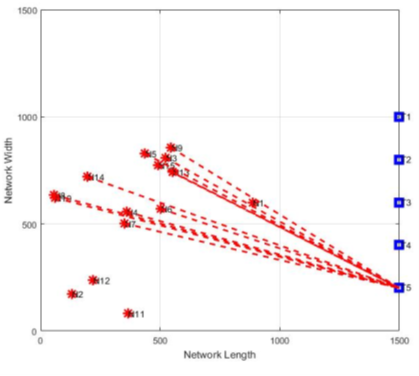
\includegraphics[height = 7cm,width = 0.7\columnwidth]{Networking-diagram.png}
    \caption{Simulations using said model and algorithm}
  \end{figure}  
\end{frame}
\begin{frame}{Figures}
  \begin{figure}[!]
    \centering
     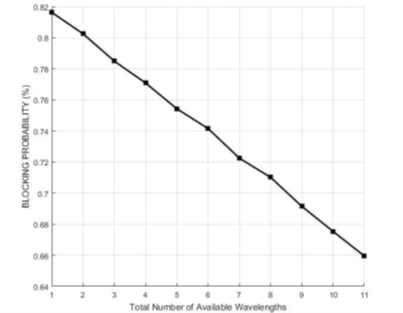
\includegraphics[height = 7cm,width = 0.7\columnwidth]{BP with lambda.png}
    \caption{Variation of BP with number of wavelength}
  \end{figure}
\end{frame}
\begin{frame}{Figures}
  \begin{figure}[!]
    \centering
     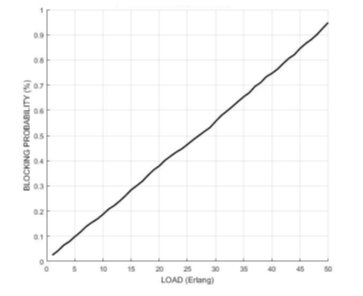
\includegraphics[height = 7cm,width = 0.7\columnwidth]{BP with load.png}
    \caption{Variation of BP with traffic}
  \end{figure}
\end{frame}
\end{document}